\chapter{Discussion}
\label{chap:9_discussion}


\section{Learning Collision Avoidance}
When designing a complex navigation policy, a combination of multiple factors ultimately shape and facilitate the convergence of the training process. Along the curriculum, we observed several features worth discussion, such as the oscillation of the average return during training, the existence of poor policy configuration spaces and the seemingly bounded timeout rates. 
In the following sections, we aim to uncover the underlying factors which could give rise to these features, and consider possible improvements.

\subsection{Oscillations and Low Returns Despite Low Collisions Rates}
Two of the most prominent features seen in almost all the figures of \cref{sec:7_learning_curriculum} are the oscillations of the average return, and the combination of low returns with low collision rates. Beginning with oscillations, we mentioned that intuitively, these can be accredited to the exploratory nature of a reinforcement learning agent, such that attempting poor actions are a part of the learning process. But, what does this mean \textit{exactly}? We can ask ourselves -- why were the oscillations so large, or why did the policy not just continue improving after finding the goal? 

These may sound like naive questions, but are in fact a part of large, central themes of deep reinforcement learning, primarily the questions of \textit{exploration} and \textit{stability} during training -- to which a multitude of algorithms have been developed to ``solve''. Taking for example the novel on-policy PPO, some of its benefits include faster training by, ``ignoring uninteresting parts of the space'' and ``faster initial planning'' \cite{suttonAndBartoBook}, better data-efficiency \cite{PPO}, and also  ``stronger convergence results'' when sampling on-policy \cite{suttonAndBartoBook} and the supposed, ``guaranteed monotonic improvement'' from trust-region based policy optimisation \cite{TRPO}.

To try and explain the oscillations, we have to remember that we have a very complicated state-action space, along with a few loss functions in e.g. actor-critics, that results in a very complex optimisation space. We can provide the common analogy that the policy space is like hills on a grassland, where we wish to perform gradient ascent to reach the highest peak. An example given in \cref{subsec:7_1_obstacle} was that we observed an early behaviour where the agent had learned to avoid obstacles by passing them always on one side. This example could correspond to a locally optimum solution for that environment -- or a hill.  
However, in progressively cluttered environments, this locally optimal solution does not hold and results in crashes that push the agent away from that locally optimum solution. In a more complicated optimisation space, the hills becomes a mountain range which have sharp maxima due to the high-dimensional optimisation space. So in this situation, if we move away from a locally optimal solution, the agent policy can either diverge if the actions performed are exceedingly poor -- resulting in high actor losses and gradient updates that push the policy completely off the mountain -- or it could find itself converging to a new locally optimum solution -- to the neighbouring mountain. But in between mountain peaks, the observed policy performance would be poor, such that we observe large dips in the average return. In addition, due to accidents and the random nature of our stochastic policy, small deviations that motivate our policy to keep exploring the policy space is inevitable.

However, this theory does not explain how the collision rate stays low in between locally optimal policies. This is a more difficult question, as we cannot simply excuse the good performance to random exploration as we did for the average return. To provide justification to this, we can attempt to explain it through the reward function.


\subsection{Converging to an Optimal Policy with Sparse Rewards}
\label{subsec:9_sparse_rewards}
The only feedback signal an agent receives while searching its complex optimisation space is the notion of the reward. We can think of the reward as the guide for providing gradients in this optimisation space, and the reward function as the one which shapes it. In hindsight, a rather clear aspect of the reward that was not apparent during its design was the problem of \textit{sparse rewards} combined with heavy penalty \textit{shaping}. Sparsity in this context refers to the amount of states in the state distribution that actually provide a reward, while shaping refers to the notion of adding extra reward terms to shape the final behaviour of the quadrotor.
In our case, the positive rewards only applied to the states very close to goal, while the added penalties could apply to all states, as seen in \cref{subsec:5_reward_function}.

This concept can therefore explain why collision rates were consistently quite low, while ``optimal'' policies were less common. Since we \textit{shape} the reward function with many penalties, the task of avoiding an obstacle is well-defined meaning that with enough experience, the agent will understand to not crash into obstacles due to its prevalent penalties. In contrast, state-action pairs that should deserve to trigger reward (by passing obstacles safely or to mark progress) do not get rewarded, which can result in the quadrotor having to sample the environment intensively in order to find those rewards to obtain gradients to push it back to a locally optimal solution space -- reflected through the significant, relatively low-frequency oscillations of the reward function.

Though this motivates us to shape the reward function more, it can be argued that ideally we wish to avoid doing so. The main reason is that reward shaping is a adds a layer of human bias on an already very complicated task, which could lead to sub-optimal performance unless those rewards were engineered by some expert in the task. Otherwise, added features could lead to unexpected consequences -- as mentioned in \cref{subsec:5_reward_function}, ``any undesired behaviour that is observed in test-time is often a consequence of a poorly designed reward function''.
Nonetheless, despite having sparse rewards, we did observe that the agent managed to learn how to solve its training task to a great extent at specific iterations, such as the best policy in for 9 obstacles in \cref{subsec:7_9_obstacles} which proved to be optimal for its task during evaluation. But then a natural follow-up would be: with such sparsity in the reward function, how did the agent learn how to perform so well across its entire state-space distribution?

A more theoretical explanation follows from the definition of the problem task, and how reinforcement learning agents learn optimal policies. We first note that an optimal policy does not need to learn how to maximise its return from all states, but only the states under the induced trajectory distribution $p_\pi$. This is important since PPO is on-policy, such that due to it limited exploration it could perform quite poorly in states uncommon under its current policy $\pi_{\bt}$. This was also observed to some extent in the large environment in \cref{fig:7_large_env_9_policy}, where the a large proportion of crashes occurred in states which were uncommon. Next, we have to recall that by definition, maximising its return means to maximise the \textit{infinite sum of discounted reward}. This means that even though we have sparse rewards, the expected return for states-action pairs far away from goal are non-zero. In fact, if we take a simple example where the reward function is just $+8$ if goal is reached, and we assume it takes 160 timesteps to reach goal (the length of our episodes), the expected return for being in its current state should be evaluated to be $8*0.99^{160} = 1.6$, where we choose the discount factor $\gamma = 0.99$. In this example, the sum of discounted rewards was simply the last timestep of the whole episode, though for our training setup the reward is much more significant since we allow the reward to be gathered until timeout (on timeout we also bootstrap the critic estimated return to the reward), while the penalties are quite low with the exception of the collision penalty. This means that while PPO is training, even though actions do not produce rewards immediately, the critic network should have an idea of the value of certain states, such that it can calculate the advantage $\widehat{A}_t$ and provide correct gradient feedback to the policy.
Therefore, if certain actions incur penalties straight away, but the trajectory ultimately leads to goal, the policy will be updated to increase the probability of doing these actions again (given that the critic did not expect them to reach goal). 

Yet, if we continue to larger and more complicated tasks, we can approach a problem where these rewards are very rarely sampled. Thus, if a policy continuously samples a trajectory where all actions lead to a collision, the critic will evaluate any action at all as bad, since the expected return is less than just remaining still. Therefore, another detail to keep in mind is that the number of timesteps cannot be too low such that the quadrotor has no time to reach goal. If we increase the episode length, the agent will be less ``rushed'' to reach the goal, and can so take more careful or elaborate routes to obtain the reward. This can also explain why we observed the timeout rates to be higher in the training plots for the 3-obstacle rate compared to the 1-obstacle, as we increased the number of timesteps from 100 to 160. 
However, the number of timesteps to set should be upper bounded, due the the discounted nature of the return.

To summarise, the expected value of states far away from rewards must be non-zero, such that gradients for actions performed in these states can be evaluated. Then to ensure this, we identify two important factors:
\begin{itemize}
    \item The number of timesteps between start and goal cannot be too large ($>400 timesteps$). Otherwise, the expected return for early states would be negative due to the heavily discounted reward and prevalence of penalties in the environment.
    \item Despite being sparse, rewards cannot be too sparse to the extent they are never experienced. Otherwise, the policy will never be able to motivate any choice of action.
\end{itemize}
To deal with the first point, we can limit the size of the environment to some maximum size or increase the discount factor to a larger value, such as 0.998 in \cite{AMPMotionPriors}.
As for the second, we can ensure that the agent always has time to reach goal by increasing the episode length some minimum value. However, this is not always necessary if we include a curriculum.


\subsection{The Role of the Curriculum}
In situations where it is desirable to have sparse rewards, we can utilise a curriculum to solve the problem. In this context, curriculum learning enables us to utilise a simple reward function for learning a complicated task by defining goals of appropriate difficulty for the current policy \cite{sparseRewards_autoGoalGeneration}. Particularly, in regards to robotic tasks, searching directly in the policy space is difficulty, because ``it deals simultaneously with complex environmental dynamics and a complex policy'' \cite{DDPG}. That is also why \cite{MotionPlanningAmongDynamicAgentsDRL2018} states that pretraining is necessary for them, or otherwise the robot wanders around and never accumulates reward. This motivates us to use a curriculum, though at the cost where the curriculum must be defined.

As we observed in the navigation evaluation studies, the learned policy could do well in for tasks it had trained for, though this had taken over 14 hours to learn. The overall initial concern is that reinforcement learning is generally sample-intensive, which is why learning a policy from scratch almost always demands the use of a simulator. This was due to the nature of optimisation, where the policy cannot learn how to solve a complicated task unless the policy repeatedly attempts some ``lucky'' sequences of actions which have high reward, and provides a large gradient to initially push the policy network in the right direction. This was also discussed in the training stage, where despite having a curriculum, choosing policies sometimes amounted to hoping for lucky combinations of good navigational ability and careful collision avoidance. 

Therefore, rather than waiting for a lucky sample trajectory, the curriculum places the policy is an ideal policy space such that the return for states in its state distribution $p_\pi$ is well defined. So for our task, with only rewards near goal, we essentially solve the problem of sparse rewards when we pretrain the policy to navigate towards goal. Intuitively, sparse rewards are defined as rewards that only influence very few states -- but under a waypoint reaching policy, the states near goal are now a large part of the policy's state distribution. 

As a result of this, we can see for example in \cref{fig:7_train_nav_1_obst}, we can create a navigation policy that knows how to avoid one obstacle over $80\%$ of times is just 30 minutes. However, learning this as quickly would not possible for end-to-end methods, unless we provided a more descriptive reward function that provided feedback to all states.


\subsection{Exploration with Parallel Sampling}
\label{subsec:9_parallel_sampling}
The underlying idea with the curriculum is that we wish to experience the most common states such that we can learn the best actions for these states quickly. In other words, we compensate for the limited exploratory nature of on-policy PPO by explicitly aiding the \textit{exploration} of the policy. Yet, simply introducing a curriculum to train a generalisable policy is not straightforward since we might artificially limit what it can explore, such that the policy converges to a \textit{strictly local} optimal solution. The benefit of parallel initialisation and sampling is that we can have varied environments, such that we facilitate exploring multiple states simultaneously. This addresses three things: first, to converge to an optimal solution we require very accurate gradients, second, for stability PPO requires that sampled data is from a very recent policy \cite{batchsizeInvariance}, and third, to learn a complex behaviour requires a wide variety of challenges \cite{RichEnvironments}.

To solve the first task, obtaining accurate gradients is synonymous with reducing variance in gradient updates. One of the most direct ways of reducing variance is through large batch sizes. Parallel sampling allows us to sample very large batch sizes, while making it computationally efficient to do so.
Second, since PPO is based on a proximal policy, our policy gradient is affected by a clipping so to not move too far from some recent policy. This requires that gradient updates are made in small increments, very often to maintain stability -- data collected from a very old policy cannot be used to calculate gradients for a new policy \cite{batchsizeInvariance}. With parallel sampling with Isaac Gym, we avoid this problem since a recent policy is always used to sample data, and through its end-to-end simulation, we avoid asynchronous update schemes such that data is only sampled after the policy has been updated.
Finally and most intuitive, by exposing our policy to many environments simultaneously, the learned behaviour can instantly be applied to all those settings. 
The mentioned benefits are also in line with \cite{song2021droneRacing}, which give credit to three main reasons for their success with PPO: 1) parallel sampling scheme 2) distributed initialisation strategy 3) random track curriculum. 



\section{Collisions in an Otherwise Optimal Policy}
Now that we have seen some of the reasons for how our agent has learned an optimal policy, we can delve into some possible reasons why certain behaviours were displayed during evaluation. Namely, we will look more closely into the causes of collisions, why our results could not readily be generalised to larger environments and possible improvements.


\subsection{Collisions by the Goal}
Evident in almost all test plots are the collisions that occur when the quadrotor are at goal. These are also the most unintuitive and difficult to explain. The first possible explanation is that due the the very parallel sampling scheme, by pure randomness in the sampled actions of the policy, the agent might accidentally collide with the ground. This can be unlikely since we observed high robustness to noise in the robustness test, and collisions were no-more likely in the noisy case than for the normal cases.

Conversely, it was observed post-testing that many of these `collisions' occurred while the quadrotor was in the air, which further added to the confusion. However, if we recall from how we detect collisions in the first place, this was either through a contact force measurement or being less than 0.2m from an obstacle. From this we can identify that the quadrotor does not necessarily have to collide with the ground, but only be within 0.2m of it. So then, since the agent has no idea of its height with respect to the global coordinate frame, only with respect to the target, we can see how collisions can occur when the target is initialised to have $z \in [0.5, 1.5]$, as the agent has only a 0.3m margin from collision when the goal is initiated at its lowest.

We can see that this explanation does make collisions near goal more plausible due to small margins, but it does not explain why the quadrotor descends so low. For this, we can recall from the evaluation studies that descending was a response to two events: either to reach goal from recently flying over an obstacle, or when reversing when the path ahead is blocked. Following this, we can imagine that when the quadrotor is very high and the goal is initialised at the bottom, this could result in collision, as mentioned in the evaluation. Furthermore, when flying through the environment, the quadrotor position is generally quite high. If we consider \cref{fig:7_hard_swapped_random}, we can see that all out of bounds events are right by goal suggesting that its position is very high even here. Furthermore, we can justify over-descent since we observe the agent over-shooting the goal, such that it has trajectory very often goes beyond the plotted targets.

Yet, by overshooting the goal, this leads to another unintended consequence, namely going to close to the edge such that it starts to reverse and descend. As already mentioned, this is a an adverse behaviour that the policy has learnt for unknown reasons -- most likely just to pass beneath simple-u obstacles. Nevertheless, we see that if the quadrotor position is quite low when it approaches the edge wall, a collision can occur too. This behaviour was also observed when we (accidentally) ran the depth robustness test with multiplicative Gaussian white noise -- since the depth images were set to 0 the quadrotor would reverse in circles until collision with the ground.

So, even though our policy is optimal in the sense of collision avoidance, it is not optimal in all aspects. To fix this problem is fortunately quite straightforward, we can increase the target and quadrotor minimum initialisation position, to be e.g. between 1.0 and 2.0 such as in Isaac Gyms \textit{Ingenuity} example.


\subsection{Difficulty of Simple-U's}
\begin{figure}[H]
    \centering
    \begin{subfigure}[b]{0.49\textwidth}
        \centering
        \captionsetup{justification=centering}
        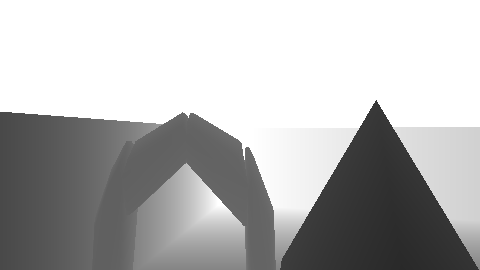
\includegraphics[width=0.98\textwidth]{figures/9_/58_0_a_pre_image.png}
        \caption{First input}
        \label{fig:58_0_a_pre_image}
    \end{subfigure} 
    \hfill
    \begin{subfigure}[b]{0.49\textwidth}
        \centering
        \captionsetup{justification=centering}
        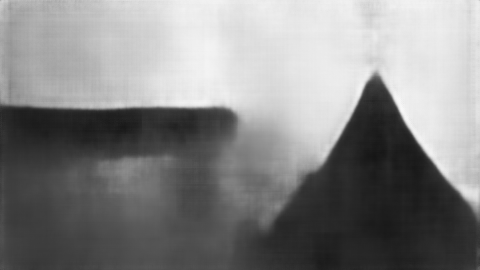
\includegraphics[width=0.98\textwidth]{figures/9_/58_0_c_vae_image.png}
        \caption{First reconstruction: a table}
        \label{fig:58_0_c_vae_image}
    \end{subfigure}
    \\
    \begin{subfigure}[b]{0.49\textwidth}
        \centering
        \captionsetup{justification=centering}
        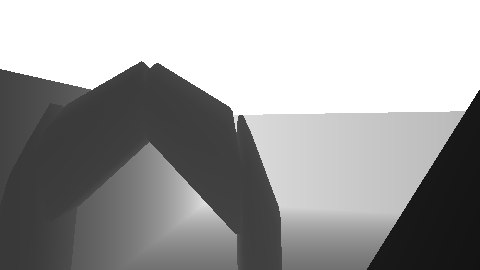
\includegraphics[width=0.98\textwidth]{figures/9_/64_0_a_pre_image.png}
        \caption{Second input}
        \label{fig:64_0_a_pre_image}
    \end{subfigure} 
    \hfill
    \begin{subfigure}[b]{0.49\textwidth}
        \centering
        \captionsetup{justification=centering}
        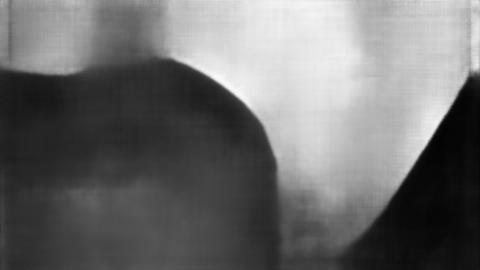
\includegraphics[width=0.98\textwidth]{figures/9_/64_0_c_vae_image.png}
        \caption{Second reconstruction: a stone}
        \label{fig:64_0_c_vae_image}
    \end{subfigure} 
    \\
    \begin{subfigure}[b]{0.49\textwidth}
        \centering
        \captionsetup{justification=centering}
        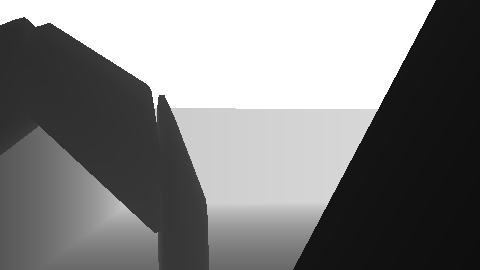
\includegraphics[width=0.98\textwidth]{figures/9_/66_0_a_pre_image.png}
        \caption{Third input}
        \label{fig:66_0_a_pre_image}
    \end{subfigure} 
    \hfill
    \begin{subfigure}[b]{0.49\textwidth}
        \centering
        \captionsetup{justification=centering}
        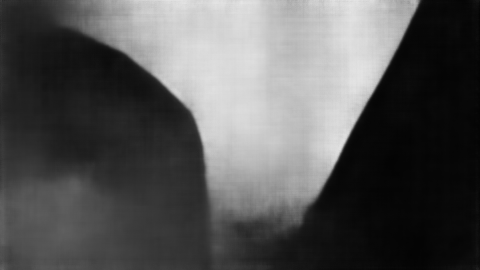
\includegraphics[width=0.98\textwidth]{figures/9_/66_0_c_vae_image.png}
        \caption{Third reconstruction: a stone}
        \label{fig:66_0_c_vae_image}
    \end{subfigure}
    \caption{Visualising the difficulty to reconstruct simple-U's. This difficulty suggests that the obstacle is not represented properly in the VAE latent space.}
    \label{fig:9_noisy_simple_u}
\end{figure}
Another challenging aspect of the quadrotor performance seemed to be the collision avoidance of the simple-U obstacles. We can also observe, for example in \cref{fig:7_easy}, that the agent opts to fly around these when it is simpler to fly through them. Intuitively we can accept this since the agent does risk colliding with the sides and the top of the arch when passing through, which is not in line with a conservative policy. However, it other cases, such as in the large environment, this behaviour led to many collisions as the quadrotor instead attempted to pass a narrow opening to the left of the simple-U instead of going through. 

To explain the difficulty of this obstacle, we found out during the depth tests that this is most likely due to the VAE not properly being able represent the simple-U in its latent space. From \cref{fig:9_noisy_simple_u}, we see that due to the filtered nature of the VAE, the arches become coloured in, such that they more closely represent a rounded stone than an arch. So the reason for not properly being able to navigate through these obstacles is not necessarily due to poor motion planning, but rather due to not being able to clearly see it.



\subsection{Lack of Normalisation in Larger Environments}
Initially, the performance of the agent in the large environments were largely unexpected. We explained that this is more likely due to a lack of generalisation, yet a simple change in environment size should be compensated for due to normalisation. Generally, if we wish to use a single architecture for a variety of tasks, we should normalise the input and outputs of the agent \cite{DDPG}. When we analysed the implementation of Isaac Gym's normalising method -- the RunningMeanStd class -- we realised the once the agent training had been completed, the means and variances of our observation and action spaces are fixed by parameters, which are then loaded in at test time.

Since we did not normalise our observation space in our environment definition, through e.g. dividing the $x$ and $y$ observations by a function of the environment size, this resulted in the quadrotor receiving much higher value observations for its position than normal. Thus, as discussed in \cref{subsec:9_parallel_sampling}, by not having the opportunity to explore this state-space leads to inferior performance. This goes in combination with our prior explanation for poor performance in the evaluation, where we reasoned that the the agent was not used to seeing obstacles so early on its state-space. 

Thus, in future implementations, we should also normalised the observation and action spaces as a function of their max value so that the performance of the policy is unaffected by changes in the environment at test time. 


\subsection{A Reactionary Policy}
Despite good performances, there is still room for improvement. As we saw in the evaluation studies, even with a near perfect score in the known environments, the policy could still crash even in the easy environment, seen in \cref{fig:7_easy}. Otherwise, we saw that in the hard environment in \cref{fig:7_hard}, the agent was subject to many pass-by and tight collisions, mainly as a result of an indirect approach and turning into a collision due to ``not remembering'' that an obstacle is right next to them. Since this is a problem that the agent cannot predict, it can also lead to inferior training performance.

From the evaluation, we observed that the policy could mend this problem itself by producing actions that do not put it too close to obstacles. However, in situations where we cannot decide on the environment before hand, such as in a random test environment in real-life, how can we prevent this?
This leads use to the main improvement that should be done with this approach, which is to included some form for internal memory. This was proposed already quite early on, in works such as \cite{pfeiffer2017perception} and implemented in \cite{worldModels2018}, where we use the RNN hidden state rather than the VAE latent code as a representation of the world. The discussion from \cite{pfeiffer2017perception} summarises this very well, stating ``we observed that the deep planner is able to avoid small dead ends if it approaches them from the outside. Once the robot enters a convex dead-end region, it is not capable of freeing itself. In addition to that, the robot’s heading sometimes fluctuates before avoiding an obstacle. This issue will be further analyzed and might be solved by using recurrent neural networks with internal memory''.
These were points were also discussed in the form of corner-situations and the concept of a favourite side for passing obstacles in the evaluation. By introducing a memory state, we also avoid this blindness problem when passing by obstacles and can more precisely pass obstacles in both pass-by scenarios but also tight ones. Moreover, since the agent being able to predict not just one time-step ahead (in a state-action mapping) policy, but also be able to predict its position and actions for future time steps, it should be able to more carefully judge which actions should be taken in the current timestep.

Generally, this approach has been widely adopted for local motion planning \cite{deepCollisionPredictorOracle, Badgr, LearningStateRepresentation} such that we can expect to gain an even better performance, particularly for the hard and larger environments. However, a paper which found that this should not be taken for granted as from their tests, only marginal performance was gained in using an LSTM hidden state, where they concluded the most important design choice was to include the use of a latent code from a VAE as a representation.



\section{VAE}


\subsection{Learning a Latent Space for Collision Avoidance}
A perhaps unseen hero
When and why does unsupervised pretraining work, chap 15.1.1 book
unsupervised pretraining is likely to be most useful when the function to be learned is extremely complicated. \cite{DeepLearningBook}



\subsection{Latent Over-Fitting}
A consequence of learning how to minimised edge reconstruction error is the possibility of over-fitting. In other words, due to the large weight of the edge loss, the VAE will indirectly learn what objects have what edges. In our training plots, we see that this is not an issue for the edge losses -- but we have to remember that the training and test sets both have the same depth data distribution, such that no new obstacles are seen at test time. Therefore, there is a possibility that the VAE has been over-fitting the depth data distribution, such that it generalises poorly to unseen ones, despite having no increase in test loss. 

This is also a possible reason why the simple-U's were reconstructed poorly, as they were not part of the input dataset. To mitigate this, we could simply ensure that our simulated dataset has the same distribution of shapes and obstacles that we will have at test time (real environments or otherwise). However, the more correct approach is to simply reduce the possibility of over-fitting by introducing some form or regularisation in the VAE network, such as Monte Carlo dropout done in \cite{dronet} and \cite{deepCollisionPredictorOracle}.







mobilenetv3-small is used in high-speed flight in the wild (instead of DroNet) has 224x3 default input size with 2.5 mil params. 

Random initialisation -- symmetry breaking \cite{LectureNotesSparseAutoencoder}.

See appendix B in VAE paper \cite{variational_bayes}. The analytic solution for KL divergence between approx posterior and prior is introduced, but the implementation in train\_vae.py was missing a .pow(2) on logvar -- saw the same in other implementations. Keras tutorial loss doesn't use analytic solution, instead just computes log of Gaussian pdfs and takes the difference (same as KL div), works well.

often we want batch norm for stability, KL div already pushes latent variables to follow normal distribution, so this is a nice side-effect during training.


binary cross-entropy does maximum likeihood estimatiion, but it assumes our data is Bernoulli distributed (black white pixels) -- pushes pixels to either 0 or 1.
MSE is maximum likelihood estimation, which is cross entropy too, but it assumes our target distribution $p(\d)$ is Gaussian. That's why it is centered around 0.5.
remember that we're minimising the KL divergence between our input data and model. VAEs specify a regularisation term that penalises p-z from deviating from Gaussian, but it does not make an assumption on p-data. This is specified in the reconstruction loss.


\section{Modular-based Approach}
It has often been assumed that standard policy search methods such as those explored in the present
work are simply too fragile to scale to difficult problems: End-to-End Training of Deep Visuomotor Policies paper, very relevant start.

Standard model-free deep RL aims to unify these challenges of representation learning and task learning into a single end-to-end training procedure. However, solving both problems together is difficult, since an effective policy requires an effective representation, and an effective representation requires meaningful gradient information to come from the policy or value function, while using only the model-free supervision signal (i.e., the reward function). As a result, learning directly from images with standard end-to-end RL algorithms can in practice be slow, sensitive to hyperparameters, and inefficient. SLAC \cite{stochastic_latent_actor_critic} intro. Opposite of navrep \cite{NavRep_unsupervised}.